%%%%%%%%%%%%%%%%%%%%%%%%%%%%%%%%%%%%%%%%%%%%%%%%%%%%%%%%%%%%%%%%%%%%%%%
%% template for II2202 report
%% original 2015.11.24
%% revised  2020.09.09
%%%%%%%%%%%%%%%%%%%%%%%%%%%%%%%%%%%%%%%%%%%%%%%%%%%%%%%%%%%%%%%%%%%%%%%
%
\documentclass[12pt,twoside,english]{article}
\usepackage[utf8]{inputenc}
\usepackage[hidelinks]{hyperref}
\usepackage{booktabs} % For \toprule, \midrule and \bottomrule
\usepackage{siunitx} % Formats the units and values
\usepackage{pgfplotstable}
\usepackage{longtable}
\usepackage{subfig}
\usepackage{graphicx}
\usepackage{courier}
\usepackage{soul}
\usepackage{adjustbox}
\usepackage[paper=a4paper,dvips,top=1.5cm,left=1.5cm,right=1.5cm,
    foot=1cm,bottom=1.5cm]{geometry}


\usepackage{todonotes}          %to provide inline and margin notes
%\usepackage[T1]{fontenc}
%%\usepackage{pslatex}
\renewcommand{\rmdefault}{ptm} 
\usepackage{mathptmx}
\usepackage[scaled=.90]{helvet}
\usepackage{courier}
%
\usepackage{bookmark}

\usepackage{fancyhdr}
\pagestyle{fancy}

%%----------------------------------------------------------------------------
%%   pcap2tex stuff
%%----------------------------------------------------------------------------
 %%\usepackage[dvipsnames*,svgnames]{xcolor} %% For extended colors
 %%\usepackage{tikz}  %% Already loaded
 %%\usetikzlibrary{arrows,decorations.pathmorphing,backgrounds,fit,positioning,calc,shapes}

%% \usepackage{pgfmath}	% --math engine
%%----------------------------------------------------------------------------
%% \usepackage[latin1]{inputenc}
\usepackage[utf8]{inputenc} % inputenc allows the user to input accented characters directly from the keyboard
\usepackage[english]{babel}
%% \usepackage{rotating}		 %% For text rotating
\usepackage{array}			 %% For table wrapping
\usepackage{graphicx}	                 %% Support for images
\usepackage{float}			 %% Suppor for more flexible floating box positioning
\usepackage{color}                       %% Support for colour 
\usepackage{mdwlist}
%% \usepackage{setspace}                 %% For fine-grained control over line spacing
%% \usepackage{listings}		 %% For source code listing
%% \usepackage{bytefield}                %% For packet drawings
\usepackage{tabularx}		         %% For simple table stretching
%%\usepackage{multirow}	                 %% Support for multirow colums in tables
\usepackage{dcolumn}	                 %% Support for decimal point alignment in tables
\usepackage{url}	                 %% Support for breaking URLs
\usepackage[perpage,para,symbol]{footmisc} %% use symbols to ``number'' footnotes and reset which symbol is used first on each page
\usepackage{siunitx}
\newcommand{\SIadj}[2]{\SI[number-unit-product={\text{-}}]{#1}{#2}}

%% \usepackage{pygmentize}           %% required to use minted -- see python-pygments - Pygments is a Syntax Highlighting Package written in Python
%% \usepackage{minted}		     %% For source code highlighting

%% \usepackage{hyperref}		
\usepackage[all]{hypcap}	 %% Prevents an issue related to hyperref and caption linking
%% setup hyperref to use the darkblue color on links
%% \hypersetup{colorlinks,breaklinks,
%%             linkcolor=darkblue,urlcolor=darkblue,
%%             anchorcolor=darkblue,citecolor=darkblue}

%% Some definitions of used colors
\definecolor{darkblue}{rgb}{0.0,0.0,0.3} %% define a color called darkblue
\definecolor{darkred}{rgb}{0.4,0.0,0.0}
\definecolor{red}{rgb}{0.7,0.0,0.0}
\definecolor{lightgrey}{rgb}{0.8,0.8,0.8} 
\definecolor{grey}{rgb}{0.6,0.6,0.6}
\definecolor{darkgrey}{rgb}{0.4,0.4,0.4}
%% Reduce hyphenation as much as possible
\hyphenpenalty=15000 
\tolerance=1000

%% useful redefinitions to use with tables
\newcommand{\rr}{\raggedright} %% raggedright command redefinition
\newcommand{\rl}{\raggedleft} %% raggedleft command redefinition
\newcommand{\tn}{\tabularnewline} %% tabularnewline command redefinition

%% definition of new command for bytefield package
\newcommand{\colorbitbox}[3]{%
	\rlap{\bitbox{#2}{\color{#1}\rule{\width}{\height}}}%
	\bitbox{#2}{#3}}

%% command to ease switching to red color text
\newcommand{\red}{\color{red}}
%%redefinition of paragraph command to insert a breakline after it
\makeatletter
\renewcommand\paragraph{\@startsection{paragraph}{4}{\z@}%
  {-3.25ex\@plus -1ex \@minus -.2ex}%
  {1.5ex \@plus .2ex}%
  {\normalfont\normalsize\bfseries}}
\makeatother

%%redefinition of subparagraph command to insert a breakline after it
\makeatletter
\renewcommand\subparagraph{\@startsection{subparagraph}{5}{\z@}%
  {-3.25ex\@plus -1ex \@minus -.2ex}%
  {1.5ex \@plus .2ex}%
  {\normalfont\normalsize\bfseries}}
\makeatother

\setcounter{tocdepth}{3}	%% 3 depth levels in TOC
\setcounter{secnumdepth}{5}
%% Acronyms
\usepackage[acronym, nopostdot]{glossaries}
\glsdisablehyper
\makeglossaries

\renewcommand{\headrulewidth}{0pt}
%%%%%%%%%%%%%%%%%%%%%%%%%%%%%%%%%%%%%%%%%%%%%%%%%%%%%%%%%%%%%%%%%%%%
%% End of preamble
%%%%%%%%%%%%%%%%%%%%%%%%%%%%%%%%%%%%%%%%%%%%%%%%%%%%%%%%%%%%%%%%%%%%
\usepackage{verbatim}
\newcommand{\detailtexcount}[1]{%
  \immediate\write18{texcount -merge -sum -q #1.tex output.bbl > #1.wcdetail }%
  \verbatiminput{#1.wcdetail}%
}
\newcommand{\quickwordcount}[1]{%
  \immediate\write18{texcount -1 -sum -merge -q #1.tex output.bbl > #1-words.sum }%
  \input{#1-words.sum} words%
}
\newacronym{HEP}{HEP}{High Energy Physics}



\sisetup{
  round-mode          = places, % Rounds numbers
  round-precision     = 4, % to 2 places
}

\title{A Review on Text Data Formats for Time Series Data}
\author{
        \textsc{Steven Shidi Zhou}
            \qquad
        \textsc{Emil Ståhl}
        \mbox{}\\
        \normalsize
            \texttt{shidi}
        \textbar{}
            \texttt{emilstah}
        \normalsize
            \texttt{@kth.se}
}
\date{\today}


\lhead{II2202}
\rhead{\date{\today}}

\makeatletter
\let\ps@plain\ps@fancy 
\makeatother

\setlength{\headheight}{15pt}
\begin{document}
%%%%%%%%%%%%%%%%%%%%%%%%%%%%
%%%%%%%% FRONT PAGE %%%%%%%%
%%%%%%%%%%%%%%%%%%%%%%%%%%%%

\begin{titlepage} % Suppresses displaying the page number on the title page and the subsequent page counts as page 1
	\newcommand{\HRule}{\rule{\linewidth}{0.5mm}} % Defines a new command for horizontal lines, change thickness here
	
	\center % Centre everything on the page
	
	%------------------------------------------------
	%	Headings
	%------------------------------------------------
	
	\textsc{\LARGE KTH Royal Institute of Technology }\\[1.5cm] % Main heading such as the name of your university/college
	
	\textsc{\Large II2202}\\[0.5cm] % Major heading such as course name
	
	\textsc{\large Research Methodology and Scientific Writing}\\[0.5cm] % Minor heading such as course title
	
	%------------------------------------------------
	%	Title
	%------------------------------------------------
	
	\HRule\\[0.4cm]
	
	{\huge A Review on Text Data Formats for\\ Time Series Data}\\[0.1cm] % Title of your document
	
	\HRule\\[1.5cm]
	
	%------------------------------------------------
	%	Author(s)
	%------------------------------------------------
	
		\begin{minipage}{0.4\textwidth}
		\begin{flushleft}
			\large
			\textit{Author}\\
			Emil \textsc{Ståhl}  % Your name
		\end{flushleft}
	\end{minipage}
	~
	\begin{minipage}{0.4\textwidth}
		\begin{flushright}
			\large
			\textit{Author}\\
		    Steven \textsc{Shidi Zhou} 
		\end{flushright}
	\end{minipage}

	%------------------------------------------------
	%	Date
	%------------------------------------------------
	
	\vfill\vfill\vfill % Position the date 3/4 down the remaining page
	
	{\large \today} % Date, change the \today to a set date if you want to be precise
	
	%------------------------------------------------
	%	Logo
	%------------------------------------------------
	
	%\vfill\vfill
	%\includegraphics[width=0.2\textwidth]{placeholder.jpg}\\[1cm] % Include a department/university logo - this will require the graphicx package
	 
	%----------------------------------------------------------------------------------------
	
	\vfill % Push the date up 1/4 of the remaining page
	
\end{titlepage}

\maketitle


\begin{abstract}
\label{sec:abstract}
\begin{center}
Data science pipelines process vast amounts of data stored in various data formats. For pipelines to be high performing, it is important to choose the right data format for the given application. Since data formats are implemented using different technologies, they may differ in how they handle different sizes of data. In this work, we investigate the read-and-write performance, file stability, as well as file storage size of some of the most popular data formats including csv, xlsx, Avro, and Parquet. The output of the thesis is a wide overview of how the performance of data formats is impacted by aspects such as file size and file corruption due to bit flips. The obtained results show that the four benchmarked data formats behave differently. Specifically, the discrepancy shows that Parquet offers the best read and write as well as file store performance. However, in the file stability benchmark, Parquet performed the worst while csv showed the most resilience against file corruption due to bit flips. This means that there is a trade-off between read/write performance, file store size, and file stability. This work shows that Parquet is the data format best fit for handling time series data. Suggestions for future work include repeating the read-and-write benchmark by utilizing the Apache Spark framework instead of Pandas as well as using a different data set other than time series data. 
\end{center} 
\end{abstract}
%%\clearpage

\pagenumbering{gobble}
\selectlanguage{english}

\clearpage
\tableofcontents
\clearpage

%%\section*{List of Acronyms and Abbreviations}
%%\label{list-of-acronyms-and-abbreviations}
%%\renewcommand{\glossarysection}[2][]{} %% skip the title
%%\printglossary[type=\acronymtype,nonumberlist]


\clearpage
\pagenumbering{arabic}

\section{Introduction}
\label{sect:introduction}
Data science pipelines process vast amounts of data stored in various data formats. In the field of the \gls{IoT} alone, there are billions of sensors and computing devices that are collecting and analyzing large amounts of personal data \cite{noauthor_state_2022}. For pipelines to be high performing, it is important to choose the right data format for your application. Since different data formats are implemented using different technologies, they may differ in how they handle different sizes of data \cite{cao_data_2017}. However, there are currently no conventions or general knowledge regarding when to use a particular data format for a given data size to optimize for performance, file stability, and file size. In this work, we are going to investigate how data science pipelines can be optimized by choosing the correct format when processing textual time series data. 


\subsection{Background}
\label{sec:introbac}
The modern society produces a vast amount of data every day across many different types of industries and pipelines. Until processed, these data are merely bits placed on a storage medium. The field of data science is focused on extracting useful knowledge from such data in order to gain a deeper understanding of a given field. Data can be stored in various formats such as csv, xlsx, Parquet, and Avro. Processing data requires many operations to be applied, such as reading, writing, and other mathematical operations. The value that data science brings places heavy demands on the performance and stability of the data formats used in data processing and storage pipelines. Related work has been done by Plase et al., who in their work "\textit{A comparison of HDFS compact data formats: Avro versus Parquet}" have benchmarked the amount of disk space these formats consume, as well as their performance in the \gls{HEP} analysis, which uses a lot of numerical data. However, the work does not benchmark read-and-write speed, file stability, or performance on time series text data. Understanding the performance advantages of different data formats in terms of read and write speed when working with time series text data is therefore of paramount importance in the data science community\cite{plase_comparison_2017, cao_data_2017}.

\subsection{Problem}
\label{sect:problem}
Analyzing the performance and stability of different data formats is key to addressing the scalability and performance challenges in which data science pipelines operate. Today, there exist more than 44 zeta bytes of data with approximately 2.5 Quintilian bytes of data being generated each day \cite{howarth_30_2022}. Data science pipelines must be highly optimized performance-wise to be able to process data at sufficient speeds and to ensure stability as well as job efficiency \cite{cao_data_2017}. Since different data formats are implemented using different technologies, they may differ in how they handle different sizes of data, which affects the performance when processing and storing the data. There are currently no conventions for when to use a particular data format for a given data size to optimize performance, file stability, and file size. Since csv, xlsx, Parquet, and Avro are all widely used in data science, it is important to have an understanding of their behavior when processing and storing data \cite{cao_data_2017}.

\subsection{Purpose}
\label{sec:purpose}
This paper aims to give the interested reader guidelines regarding how to choose a data format when working with textual time series data. The purpose of this work is to analyze the performance of the csv, xlsx, Parquet, and Avro data formats by
quantifying their read/write speed, file stability, and file size to determine which data format is the most optimal when working with textual time series data. By analyzing the performance of these data formats under different pipeline conditions, such as file size, one can use this work to tailor data science pipelines to optimize performance. The results are potentially of interest to general data scientists, stock market traders, developers of big data frameworks, and the open-source community.

\clearpage
\subsection{Research questions and hypothesis}
Considering the background and problem discussion, this work will treat the following questions. 
\label{sect:questions}
\begin{itemize}
    \item \textbf{RQ1} How do the csv, xlsx, Parquet, and Avro data formats differ in terms of read and write performance when processing textual time series data?
    \item \textbf{RQ2} How do the csv, xlsx, Parquet, and Avro data formats differ in terms of resilience against file errors due to random bit flips when storing textual time series data?
    \item \textbf{RQ3} How do the csv, xlsx, Parquet, and Avro data formats differ in terms of file size when storing textual time series data?
\end{itemize}

With this work, we expect there to be an advantageous data format for a given file size when working with textual time series data. The row-based Avro format should provide advantages in performance with regard to simple operations such as read/write speeds when compared to csv, xlsx, and Parquet. For larger time series data sets, the Apache Parquet format should provide better performance. Regarding file stability we expect csv to be more resilient against file errors due to that it is uncompressed.


\subsection{Benefits, Sustainability, and Ethics}
\label{sect:benefits}
Many possible benefits may result from understanding the performance and stability of different data formats in data science. Regarding sustainability, the biggest contribution in this matter would be to reduce the energy consumption of data science pipelines. Smaller file sizes result in less network bandwidth being used, as well as less waiting time for the cluster to load and process data. This would hopefully be able to free up more machines which results in less energy being consumed and combined with works such as "Green network control" it would have a meaningful environmental impact \cite{cao_data_2017}. Sustainable energy, meaning less consumption, is one of the Sustainable Development Goals created by the United Nations \cite{bexell_responsibility_2017}. Therefore, this work could result in positive sustainability impacts. Regarding ethics, there exist several areas that are interesting from an ethics perspective. For example, showing limitations in how a specific data format or software performs and functions may cause harm to the developers behind it. This may deter people from using it which may cause harm to the copyright holder or third-party software that relies on the data format in question. However, benchmarking is widely accepted in the software community and is often welcomed by the users and developers behind the software that is being tested. Therefore, we argue that there are no major ethical problems that deter us from researching this area \cite{bexell_responsibility_2017}. 

  
\subsection{Methodology}
\label{sect:intromethod}
The decision of methodology is important in a scientific study. In this work, the research method used is defined as \textit{experimental} since the method focuses on finding aspects that affect the choice of data format when working with textual time series data \cite{hakansson_portal_2013}. Moreover, the research is also \textit{applied} since it makes use of the code for the data formats that we benchmark as well as libraries and existing methodologies, which means that the methodology is based on work performed by other researchers and developers \cite{hakansson_portal_2013, blomer_quantitative_2018}. With this in mind, the methodology used to perform this work consists of the choice and configuration of a benchmarking environment, a method for performing the experiments, and an evaluation method to analyze and evaluate the system itself. The chosen method should fulfill the purpose and goal of this thesis, which is to analyze the performance of different data formats \cite{hakansson_portal_2013}.

\subsection{Delimitations}
\label{sect:delimit}
Due to the scope of this project as well as our knowledge and available resources, a set of delimitations are needed for this work. The delimitations can be constricted to those regarding the application of the data formats to be benchmarked. As the application may influence the choice of data format, we have decided to delimit our work to only benchmark the data formats when working with textual time series data using the Pandas Python library. 

\subsection{Outline}
\label{sect:outline}
This paper is organized as follows. Chapter \ref{sect:introduction} gives an introduction to the work where the background is briefly explained. In addition to this, the purpose, the goal, and the methodology used are shortly explained along with its connection to ethics and sustainability. Chapter \ref{sect:theoryframework} is a recess of the theoretical framework and literature used in our work. Further on, Chapter \ref{sec:method} describes the methodologies and methods used to perform the work, which includes the benchmarking environment and metrics. Next, Chapter \ref{sec:results} presents the results of the performed benchmarks, mainly focusing on the performance and stability of the data formats and how these differ in-between file sizes. Chapter \ref{sec:discussion} analyses and discusses the results. In other words, what the results mean and why they look the way that they do. We also discuss how the experiments could be changed to improve the accuracy and reliability of the benchmarks. Finally, Chapter \ref{sec:conclusion} presents a conclusion of the work in relation to its purpose and goal, as well as potential future work that can be performed in order to improve the conclusions of this work.


\section{Theoretical framework}
\label{sect:theoryframework}
There are two types of data storage, row-based and column-based data formats. Row-based data stores are considered the traditional approach where we data is written one row at a time. This makes it very easy to insert new data or modify an existing record. However, with a row-based store, more data is read than is needed resulting in overhead. Column-based data, on the other hand, writes the data vertically by column. The column-based approach ensures that you only need to read the data you are interested in. However, the downside of this method is that it requires multiple accesses in order to write the records since their columns are distributed in different sections. Figure \ref{fig:rowvscolumn} below is a visual representation of the description above (Graph replicated from the presentation "The future of column-oriented data processing with Arrow
and Parquet") \cite{jack_future_nodate, cao_data_2017}. 


\begin{figure}[!h]
  \centering
  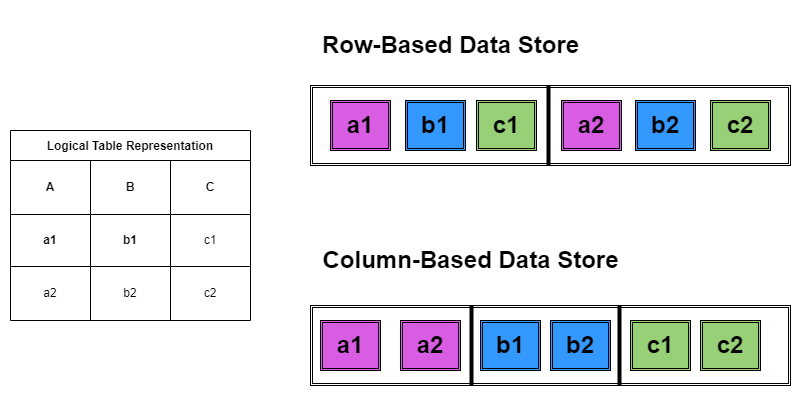
\includegraphics[width=0.7\textwidth]{img/concept.png}
  \caption{Row-based Data Store vs column-based data store. Replicate from \cite{jack_future_nodate}}
  \label{fig:rowvscolumn}
\end{figure}

\subsection{Column-based data formats}

The columnar data formats are a popular choice for fast analytic workloads. As opposed to row-oriented storage, columnar storage can significantly reduce the amount of data fetched from disk by allowing access to only the columns that are relevant to the particular query or workload. Moreover, columnar storage combined with efficient encoding and compression techniques can drastically reduce the storage requirements without sacrificing query performance \cite{floratou2018columnar}. It is worth noting that columnar data formats are suitable for large data volumes and read-only intensive workloads \cite{jack_future_nodate, cao_data_2017}. 

\subsubsection{Parquet}
Apache Parquet is a column-based serialization format mainly used in the Hadoop ecosystem, regardless of the choice of data processing framework, data model, or programming language \cite{vohra_apache_2016}. Parquet is built to support very efficient compression and encoding schemes. Instead of simply flattening the nested namespaces, it uses the record shredding and assembly algorithm described in the Dremel paper\cite{36632}. Multiple projects have demonstrated the performance impact of applying the right compression and encoding scheme to its data. Some projects, such as WikiParq, is an interesting project that builds on top of the Parquet format to tabulate and package the Wikipedia corpora\cite{klang_wikiparq_2016}. Its content can then be extracted by querying the database to obtain the exact information the user needs. Besides the points above, Parquet also allows for compression schemes to be specified on a per-column level, and is future-proofed to allow adding more encoding as they are invented and implemented \cite{vohra_apache_2016, cao_data_2017}.

\subsection{Row-based data formats}
Row-based data formats are ideal for visual data representation as well as transnational query. Examples of data formats used for visual data representation are csv and xlsx. Row-based formats are also very efficient and suitable for smaller data volumes. Below follows a presentation of each row-based data format that is to be benchmarked \cite{vohra_apache_2016_avro, cao_data_2017}.

\subsubsection{Avro}
Apache Avro is a compact binary data serialization format that provides various data structures and row-wise serialization\cite{vohra_apache_2016_avro}. Avro uses the JSON notation schema to serialize and deserialize data. Unlike some other similar systems, such as Google Protobuf, Avro does not require code generation and uses dynamic typing. Data are not tagged because the schema is accompanied with the data, resulting in a more compact data file. Avro supports versioning, so different versions of Avro data files can coexist along with their schemes. Since Avro is an Apache open-source project, many Apache projects support the Avro format such as Apache Hive, which provides support to store a table as Avro. Apache Flume supports Avro as input and output \cite{vohra_apache_2016, vohra_apache_2016_avro, cao_data_2017}. 

\subsubsection{CSV}
\gls{CSV} is a very simple format where each record is located on a separate line, delimited by a line break (CRLF) \cite{shafranovich_common_2005}. Although simple, the format has been used to exchange and convert data between various spreadsheet programs. It is also very widely used as the format for storing and distributing data in the open-source data science community \cite{shafranovich_common_2005, cao_data_2017}.

\subsubsection{Open Office XML-based spreadsheet format-XLSX}
The Open Office XML-based spreadsheet format that uses .xlsx as a file extension has been the default format produced for new documents by Microsoft Excel versions since Excel 2007 \cite{noauthor_xlsx_2022}. The format was designed to be equivalent to the binary .xls format produced by earlier versions of Microsoft Excel \cite{noauthor_xlsx_2022, cao_data_2017}. 

\subsection{Previous comparative studies}
Several previous studies have done research in this field. For example, Plase et al. compared Avro and Parquet with respect to text formats to evaluate the performance of the data queries \cite{plase_comparison_2017}. Different data query patterns have also been evaluated in this study. Blomer performed a quantitative review on some common data formats, including Parquet and Avro, with respect to \gls{HEP} datasets, which consist of n-tuples and \glspl{AOD}, and lots of numerical data\cite{blomer_quantitative_2018}. Todor Ivanov and Matteo Pergolesi have in a journal article reasoned about the impact of using columnar-based file formats with SQL for Hadoop Engine performance, mainly comparing the ORC format vs Parquet \cite{ivanov_impact_2020, cao_data_2017}.


\section{Methodology}
\label{sec:method}
In this chapter, we explain the different parts of the theoretical method used to benchmark the performance limits of the various data formats. We are going to execute three separate experiments, one corresponding to each of the research questions mentioned in \ref{sect:questions}. The data set that is to be used in this study is the Google Covid-19 Open Data \cite{noauthor_covid-19_nodate}. The data is available in \gls{CSV} and JSON formats. The source of this data set comprises authoritative sources, as well as volunteers and contributors. The Google Covid-19 dataset has multiple tables, but we are only going to use the aggregated table in this study. The aggregate table has a full version and subsets that provide only the data for the most recent day \cite{noauthor_covid-19_nodate}. The full version, named aggregated\_full.csv, is around 20 GB in size, and a subset version called v3-latest, named aggregated.csv, has a size of 24 MB. For a more rapid test and result collection, we are going to use the v3-latest version to do most of our benchmark operations. The v3-latest data set is going to be cut to have the size of 1 MB, 5 MB, 10 MB, 20 MB, and 24 MB and then be converted into the different file formats that are to be benchmarked in this work. Those files are then used for the read/write speed benchmark and file stability benchmark. For the benchmark of file store size, we will additionally convert the full version of the data, which weighs in at 20 GB, into other file formats and observe the file size changes. 


\subsection{Benchmarking environment}
The chosen benchmark environment to perform the experiments is Google Colab, which allows anyone to write and execute arbitrary Python code through the browser and is especially well suited for machine learning, data analysis, and education \cite{noauthor_google_2022}. We are going to write our benchmark scripts in the Python programming language since it is one of the most used languages in data science. Our Python code is going to automatically and empirically benchmark the read and write performance of the data formats by iteratively performing these operations 1,000 times and taking the average elapsed time that was required for the operation to finish. We will also be using some common Python packages such as the Pandas library for this experiment. The Google Colab environment has the following technical specifications \cite{noauthor_google_2022}:

\begin{itemize}
    \item CPU model name: Intel(R) Xeon(R) CPU @ 2.20GHz
    \item CPU cores: 2
    \item Available RAM: 12 GB
    \item Codec: Python\_snappy-0.6.1-cp37
    \item Python Version: 3.7.14
    \item Python Pandas Version: 1.3.5
    \item Python Fastavro Version: 1.6.1
    \item Python Snappy Version: 0.6.1
\end{itemize}

\subsection{Read \& Write Performance}
\label{read_write_performance}
For the read-and-write performance tests, we take the v3-latest version of the Covid-19 data, as well as the subsets of the data generated from it. We use the Pandas library to help us with the read-and-write benchmark. For reading and writing Avro files, we combine Pandas and fastavro since Pandas does not provide direct support for Avro. Specifically, Avro files are read using the fastavro package and then converted to a Pandas dataframe afterward. Likewise, for writing, we first convert the Pandas dataframe to records, which is a list of dictionaries, and then use fastavro to help write those into an Avro file. It is worth noting that for Avro and Parquet file formats, they offer different compression codecs, in this study we are going to use the snappy codec for both formats. To address potential bias during data collection, the benchmark program is run 1,000 times in the Google Colab environment. 

\subsection{File stability}
\label{File-stability-method}
For the file stability tests, we are going to programmatically flip random bits in the files and check their resilience and ability to operate normally. This is to replicate the experiment of file stability done by Blomer with respect to \gls{HEP} datasets, but for textual time-series data \cite{blomer_quantitative_2018}. For flipping bits in the files, we make use of the bit-flipping software written by Antoine Grondin, and is available on GitHub \cite{grondin_bitflip_2022}. The software lets us randomly flip one bit of a file. The range of possible outcomes of reading files with flipped bits consists of no change at all to a potential crash of the reading operation. For the cases where there are errors reading the file, we do another check where we compare the original file with the file that had a random bit flip; if these files have identical entries the outcome is reported as 'no effect'. However, if the file entries are not equal, the outcome is recorded as an 'undetected effect'. This procedure is executed iteratively 100 times, where we increment a counter for each possible outcome every time that specific outcome occurs, the results are saved to an excel spreadsheet that is shown in Table \ref{File-stability-benchmark} of Section \ref{sect:file-stability-results}.

\subsection{File store size}
For this benchmark, since we have already created all the subset data we simply measure the size of the converted file formats. Additionally, we are also going to try to convert the 20 GB full version of the Covid-19 data into the other file formats, and observe the file size changes.

\section{Results}
\label{sec:results}
This chapter presents the results of the benchmarks performed.

\subsection{Read/write performance}
Due to the amount of data and the length of the tables, the results of the various read and write performance benchmarks for our files are shown in tables in Appendix \ref{readappendix} and \ref{writeappendix}. The first row of each of these tables shows the filename of the benchmarked file, while each respective column shows the time in seconds it took to read the given file. These data are used to produce the summary tables and figures below. For the read benchmark shown in figure \ref{fig:read_benchmarks}, the sub-figure of xlsx benchmark in section \textit{b} is a lot smoother compared to the rest of the sub-figures, this is due to that the benchmark time for xlsx is significantly longer compared to the other file format benchmarks. For example, each read of the xlsx file named "aggregated(v3-latest)" which is around 24.1 MB in size takes an average of 172 seconds to finish. This means that if we proceed with the planned 1,000 iterations of each benchmark, it would take 48 hours to benchmark only the largest file. Therefore, we have chosen to benchmark it only 10 times for xlsx only. In the same situation as with the Avro benchmark in sub-figure \textit{c}, the benchmark for the larger files, named aggregated\_20MB and aggregated(v3-latest), are only run 100 times instead of 1,000. Figure \ref{fig:read_benchmarks_summary} presents the summary of the results of the read benchmark using the Python Pandas library. As shown in sub-figure \textit{a}, the xlsx file format shows significantly more time to finish reading compared to the other file formats, and the trend continues as the file size increases, suppressing the other file format metrics. After excluding the xlsx format, it becomes clear that the Parquet format has the best read performance compared to the rest of the benchmarked file formats since the read time increases at a very slow rate as the file size grows bigger.

\clearpage
\begin{center}
    %\caption{CSV Pandas Read Benchmark}
    \label{table:tablereadsummary}
   \pgfplotstabletypeset[
      multicolumn names, % allows to have multicolumn names
      col sep=comma, % the seperator in our .csv file
      begin table=\begin{longtable},
      end table=\end{longtable},
      %columns={$file\_size$, csv\_mean, xlsx\_mean, avro\_mean, parquet\_mean}
      display columns/0/.style={
        column name=File Size, % name of first column
        column type={l},string type},  % use siunitx for formatting
      display columns/1/.style={
        column name=CSV Mean,
        column type={S},string type},
      display columns/2/.style={
        column name=XLSX Mean,
        column type={S},string type},
      display columns/3/.style={
        column name=Avro Mean,
        column type={S},string type},
      display columns/4/.style={
        column name=Parquet Mean,
        column type={S},string type},
      every first column/.style={column type/.add={|}{}},	% style the first column
      every head row/.style={
        before row={
        \caption{Pandas Read Benchmark}%
        \endfirsthead
        \toprule
        }, % have a rule at top
        after row={%
            \si{\string} & \si{\second}& \si{\second}& \si{\second}& \si{\second}\\ % the units seperated by &
            \midrule} % rule under units
            },
        every last row/.style={after row=\bottomrule} % rule at bottom
    ]{tables/pandas_read_result_summary.csv} % filename/path to file
\end{center}
 
\begin{figure}[H]%
    \centering
    \subfloat[\centering  CSV ]{{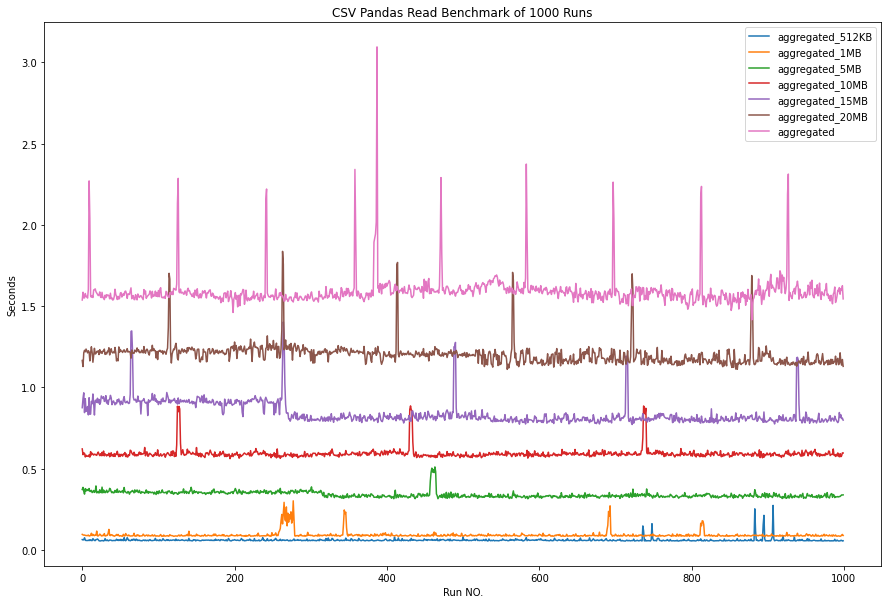
\includegraphics[width=8cm]{img/csv_read.png} }}%
    \subfloat[\centering XLSX ]{{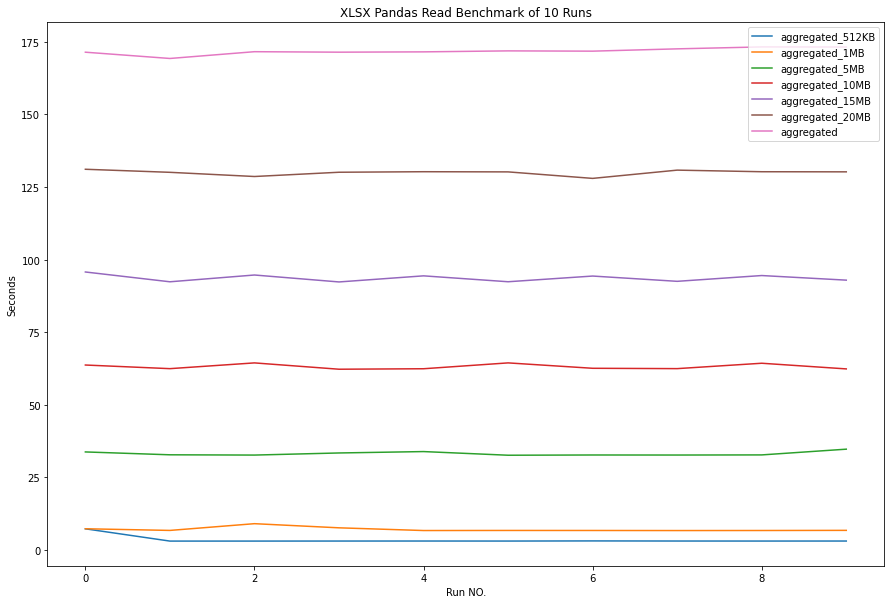
\includegraphics[width=8cm]{img/xlsx_read.png} }}%
    \quad
    \subfloat[\centering  Avro ]{{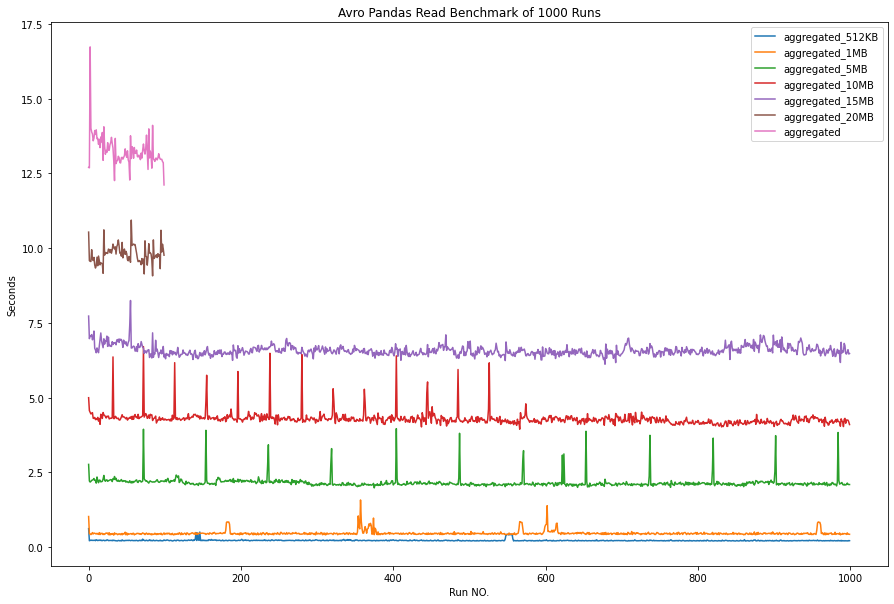
\includegraphics[width=8cm]{img/avro_read.png} }}%
    \subfloat[\centering Parquet ]{{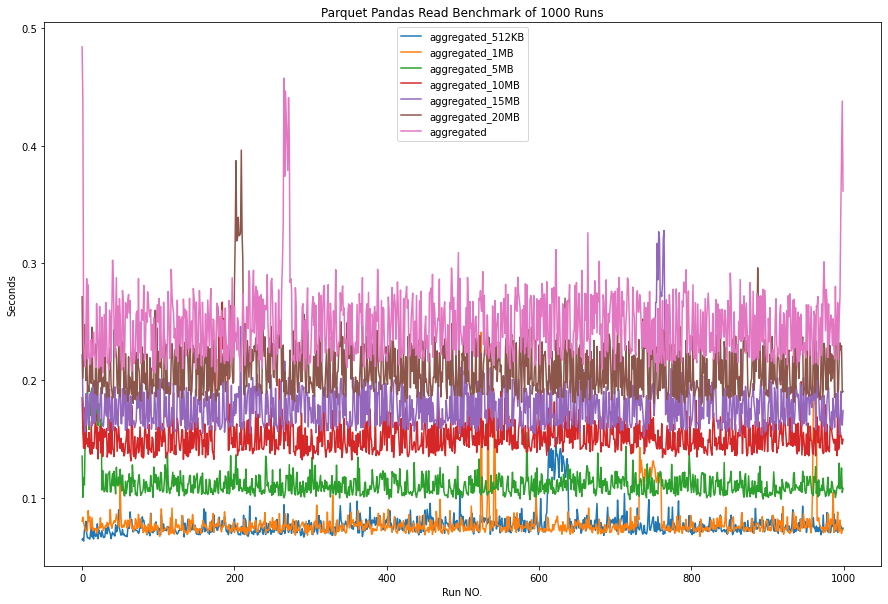
\includegraphics[width=8cm]{img/parquet_read.png} }}%
    \caption{Pandas Read Benchmark for 4 different file formats, X-axis shows each runs up to 1000th run, Y-axis shows the time it takes for each run, measured in seconds. Sub-graph b looks smooth due to the number of iterations being 10 instead of 1000, and sub-graph c has cut off for bigger file sizes because for those it was only run the benchmark 100 times instead of 1000 due to time limitation}%
    \label{fig:read_benchmarks}%
\end{figure}

\begin{figure}[H]%
    \centering
    \subfloat[\centering Read Benchmark Summary ]{{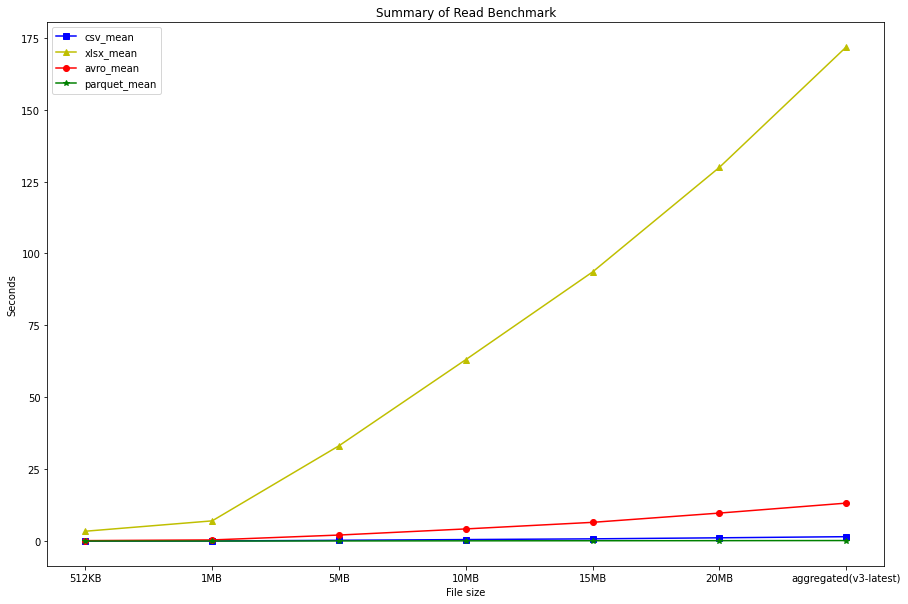
\includegraphics[width=8cm]{img/read.png} }}%
    \qquad
    \subfloat[\centering Read Benchmark Summary excluding XLSX file format]{{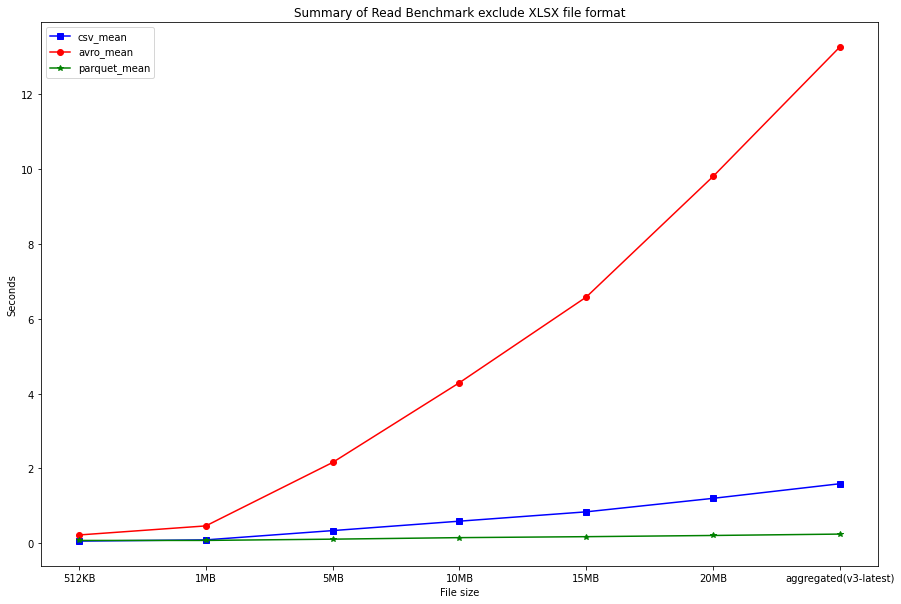
\includegraphics[width=8cm]{img/read_exlude_xlsx.png} }}%
    \caption{Summary of read benchmark using Panda for 4 different file formats, the X-axis shows the file size, starting with 0.5MB up to 24.1MB (aggregated v3-latest), while the Y-axis shows the average time it took to read the file measured in seconds}%
    \label{fig:read_benchmarks_summary}%
\end{figure}

For the write benchmark, in figure \ref{fig:write_benchmark}, the xlsx benchmark in section \textit{b} shows the same situation as its read counterpart. Meaning that we have chosen to benchmark it only 10 times for xlsx only. Due to time limitations for the Avro benchmark in sub-figure \textit{c}, the benchmarks for all sizes are only run 100 times instead of 1,000. Figure \ref{fig:write_benchmark_summary} presents a summary of the results of the write benchmark using the Python Pandas library. As shown in sub-figure \textit{a}, the xlsx file format takes significantly more time to finish writing compared to the other file formats, and the trend is only getting worse as the file size increases, suppressing the other file format's metrics. After excluding the xlsx format it becomes clear that Parquet format also has the best write performance compared to the rest of the benchmarked file formats, surprisingly the Parquet write time does not suffer as the file size increases.

\begin{center}
    %\caption{CSV Pandas Read Benchmark}
    \label{table:tablewritesummary}
   \pgfplotstabletypeset[
      multicolumn names, % allows to have multicolumn names
      col sep=comma, % the seperator in our .csv file
      begin table=\begin{longtable},
      end table=\end{longtable},
      %columns={$file\_size$, csv\_mean, xlsx\_mean, avro\_mean, parquet\_mean}
      display columns/0/.style={
        column name=File Size, % name of first column
        column type={l},string type},  % use siunitx for formatting
      display columns/1/.style={
        column name=CSV Mean,
        column type={S},string type},
      display columns/2/.style={
        column name=XLSX Mean,
        column type={S},string type},
      display columns/3/.style={
        column name=Avro Mean,
        column type={S},string type},
      display columns/4/.style={
        column name=Parquet Mean,
        column type={S},string type},
      every first column/.style={column type/.add={|}{}},	% style the first column
      every head row/.style={
        before row={
        \caption{Pandas Write Benchmark}%
        \endfirsthead
        \toprule
        }, % have a rule at top
        after row={%
            \si{\string} & \si{\second}& \si{\second}& \si{\second}& \si{\second}\\ % the units seperated by &
            \midrule} % rule under units
            },
        every last row/.style={after row=\bottomrule} % rule at bottom
    ]{tables/pandas_write_result_summary.csv} % filename/path to file
 \end{center}
 
 \begin{figure}[H]%
    \centering
    \subfloat[\centering  CSV ]{{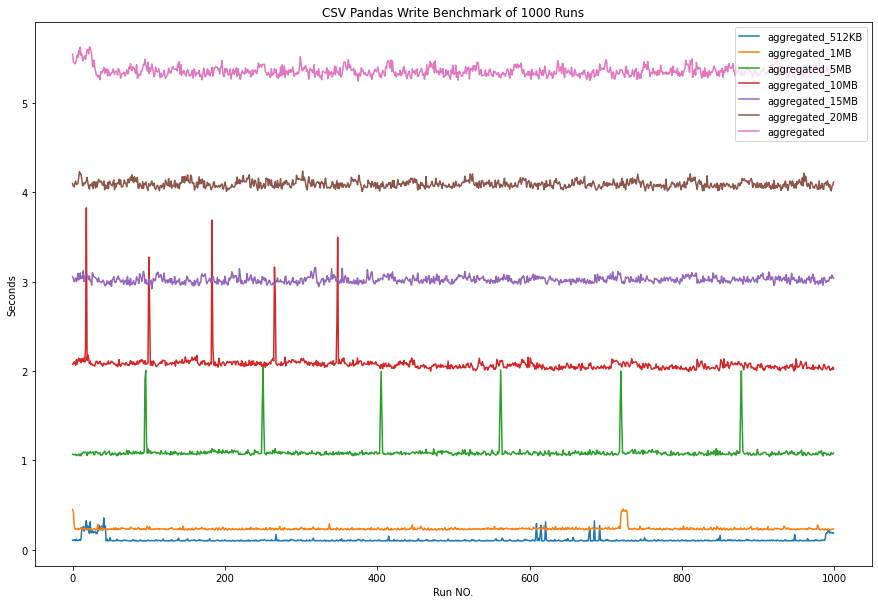
\includegraphics[width=8cm]{img/csv_write.png} }}%
    \subfloat[\centering XLSX ]{{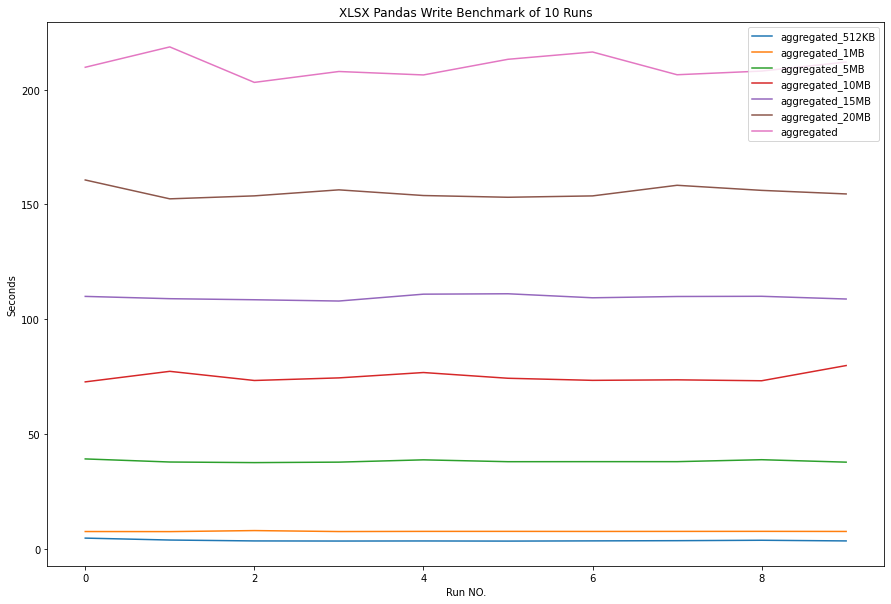
\includegraphics[width=8cm]{img/xlsx_write.png} }}%
    \quad
    \subfloat[\centering  Avro ]{{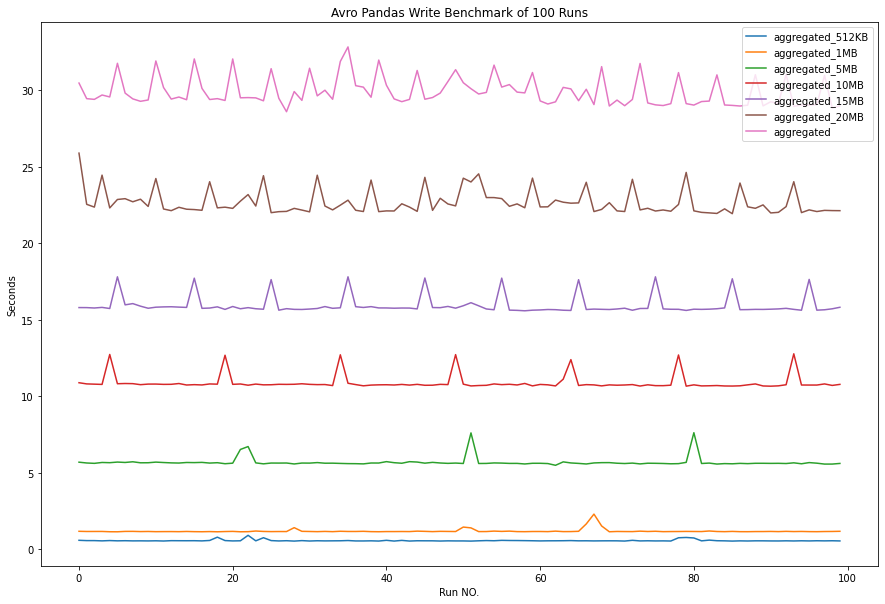
\includegraphics[width=8cm]{img/avro_write.png} }}%
    \subfloat[\centering Parquet ]{{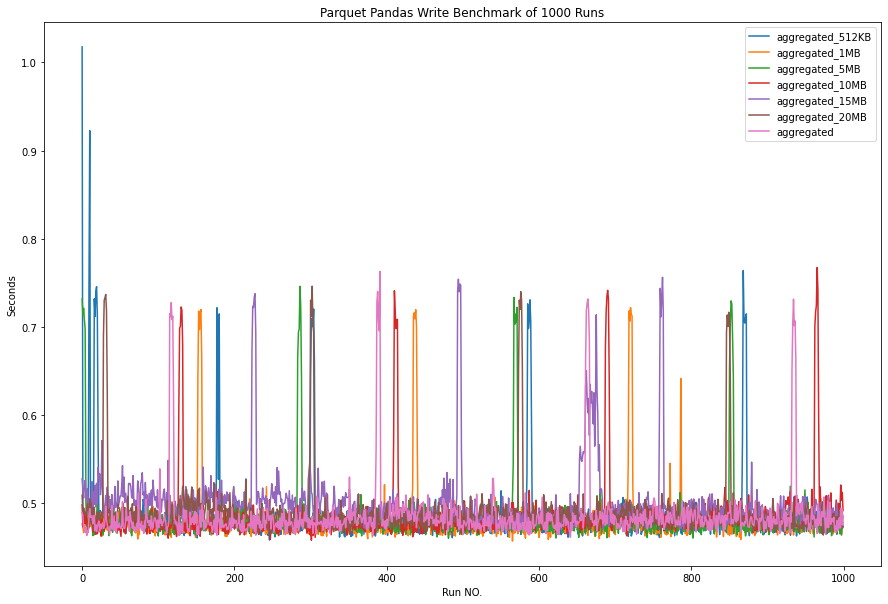
\includegraphics[width=8cm]{img/parquet_write.png} }}%
    \caption{Pandas write benchmark for 4 different file formats, the X-axis shows each run up to the 1,000th run. The Y-axis shows the time it takes for each run measured in seconds. Sub-graph \textit{b} looks smooth due to that the number of iterations is 10 instead of 1,000. Sub-graph \textit{c} also looks smoother compared to the sub-graph \textit{a} and \textit{b} because the number of iterations are  100 times instead of 1,000.}%
    \label{fig:write_benchmark}%
\end{figure}

\begin{figure}[H]%
    \centering
    \subfloat[\centering Write Benchmark Summary ]{{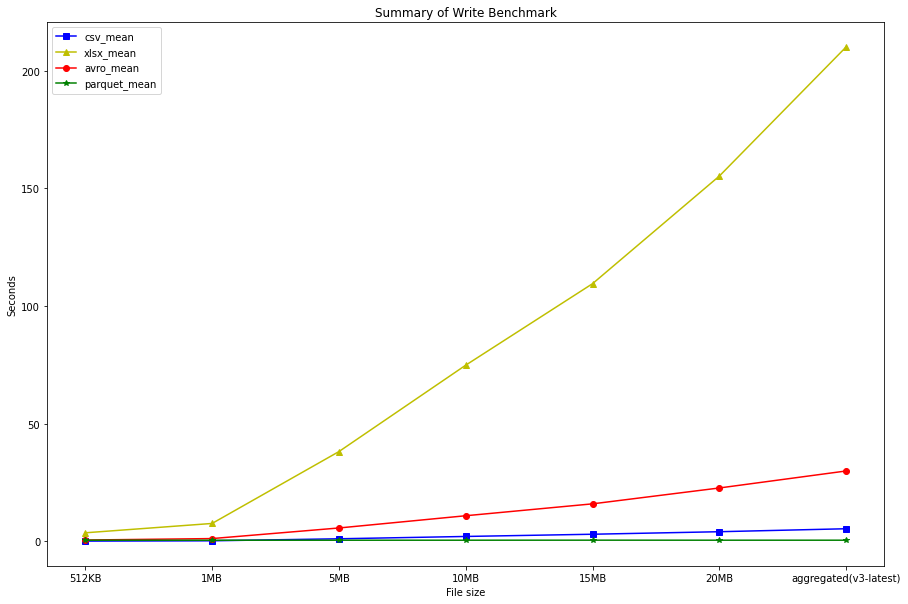
\includegraphics[width=8cm]{img/write.png} }}%
    \qquad
    \subfloat[\centering Write Benchmark Summary excluding XLSX file format]{{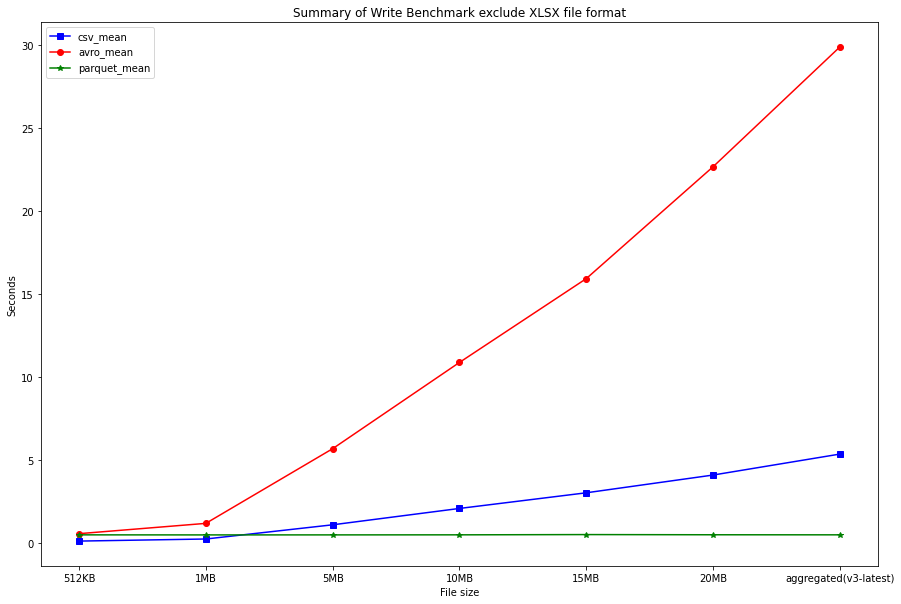
\includegraphics[width=8cm]{img/write_exlude_xlsx.png} }}%
    \caption{Summary of write benchmark using Pandas for 4 different file formats, the X-axis shows the file size starting with 0.5MB up to 24.1MB (aggregated v3-latest). The Y-axis shows the average time it took to write the file measured in seconds}%
    \label{fig:write_benchmark_summary}%
\end{figure}

\subsection{File stability}
\label{sect:file-stability-results}
 In this section, we present data from our benchmark experiment regarding the file stability explained in Section \ref{File-stability-benchmark}. Due to the significant time it takes to benchmark the xlsx format, we have excluded it from this benchmark. Table 3 shows the result of flipping a random bit in each of the files we benchmark. The first column shows the filename, while the remaining columns specify the outcome of the benchmark, ranging from \textit{Error}, \textit{No effect}, and \textit{Undetected effect}. When examining the data in Table \ref{sect:file-stability-results}, we notice that the csv files experience considerably fewer errors compared to Avro and Parquet. This is discussed in further detail in Section \ref{sec:discussion}.
\begin{center}
    \label{File-stability-benchmark}
   \pgfplotstabletypeset[
      multicolumn names, % allows to have multicolumn names
      col sep=comma, % the seperator in our .csv file
      begin table=\begin{longtable},
      end table=\end{longtable},
      %columns={$file\_size$, csv\_mean, xlsx\_mean, avro\_mean, parquet\_mean}
      display columns/0/.style={
        column name=File Name, % name of first column
        column type={l},string type},  % use siunitx for formatting
      display columns/1/.style={
        column name=File Type,
        column type={l},string type},
      display columns/2/.style={
        column name=Error,
        column type={l},string type},
      display columns/3/.style={
        column name=No effect,
        column type={l},string type},
      display columns/4/.style={
        column name=Undetected effect,
        column type={l},string type},
      every first column/.style={column type/.add={|}{}},	% style the first column
      every head row/.style={
        before row={
        \caption{Results of random bit flip when reading file}%
        \endfirsthead
        \toprule
        }, % have a rule at top
        after row={%
            \midrule} % rule under units
            },
        every last row/.style={after row=\bottomrule} % rule at bottom
    ]{tables/stability.csv} % filename/path to file
 \end{center}

\begin{figure}[h]
\centering
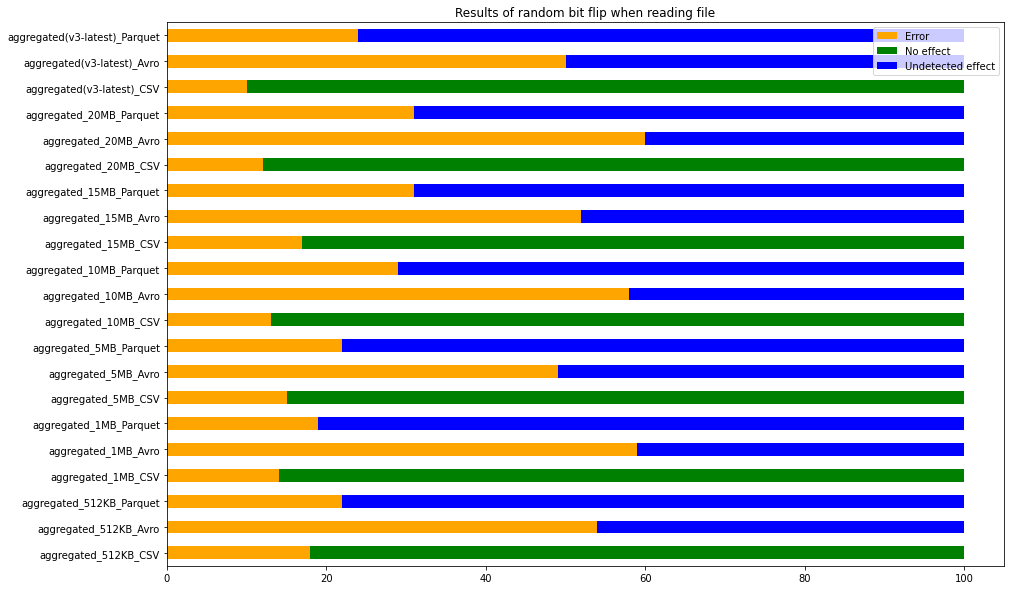
\includegraphics[scale=0.5]{img/stability.png}
\caption{Summary of file stability benchmark using Pandas for 3 different file formats including Parquet, Avro, and csv). The X-axis shows the number of runs, as well as the percentage since total of 100 runs, that were performed for each file. The Y-axis shows the file size and format, starting with 0.5MB up to 24.1MB (aggregated v3-latest)}
\label{fig:x cubed graph}
\end{figure}

\subsection{File Store Size}
The file size benchmark shown in Table 4 shows the file sizes of each file format when converted from csv format. Figure \ref{fig:size_summary} provides a visualization of the table. Since the file size difference is too large, "aggregated\_full" is therefore visualized in sub-figure \textit{b} instead of merging it with sub-figure \textit{a}. Furthermore, xlsx for "aggregated\_full" is not shown in sub-figure \textit{b} because of the lack of an effective method to convert a 20 GB csv file into xlsx format. 


\clearpage
\begin{center}
    %\caption{CSV Pandas Read Benchmark}
    \label{tablesizesummary}
   \pgfplotstabletypeset[
      multicolumn names, % allows to have multicolumn names
      col sep=comma, % the seperator in our .csv file
      begin table=\begin{longtable},
      end table=\end{longtable},
      %columns={$file\_size$, csv\_mean, xlsx\_mean, avro\_mean, parquet\_mean}
      display columns/0/.style={
        column name=File Name, % name of first column
        column type={l},string type},  % use siunitx for formatting
      display columns/1/.style={
        column name=CSV (MB),
        column type={l},string type},
      display columns/2/.style={
        column name=XLSX (MB),
        column type={l},string type},
      display columns/3/.style={
        column name=Avro (MB),
        column type={l},string type},
      display columns/4/.style={
        column name=Parquet (MB),
        column type={l},string type},
      every first column/.style={column type/.add={|}{}},	% style the first column
      every head row/.style={
        before row={
        \caption{File Store Size Benchmark}%
        \endfirsthead
        \toprule
        }, % have a rule at top
        after row={%
            \midrule} % rule under units
            },
        every last row/.style={after row=\bottomrule} % rule at bottom
    ]{tables/file_size.csv} % filename/path to file
 \end{center}
 
 \begin{figure}[H]%
    \centering
    \subfloat[\centering File Size Benchmark Summary ]{{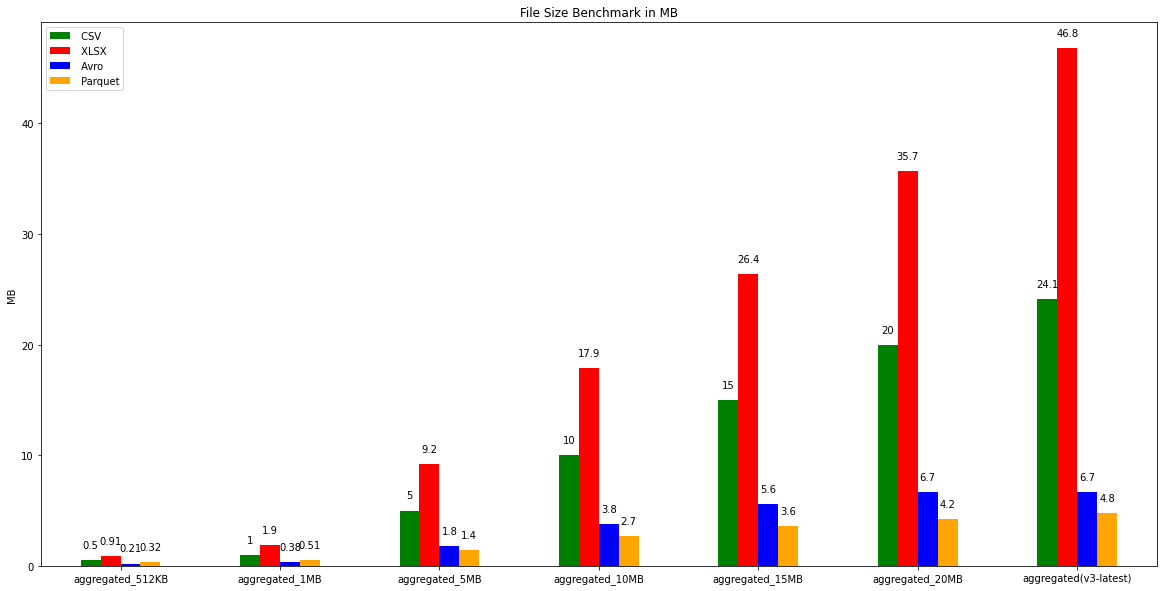
\includegraphics[width=12cm]{img/size.png} }}%
    \qquad
    \subfloat[\centering File size benchmark summary for full data format]{{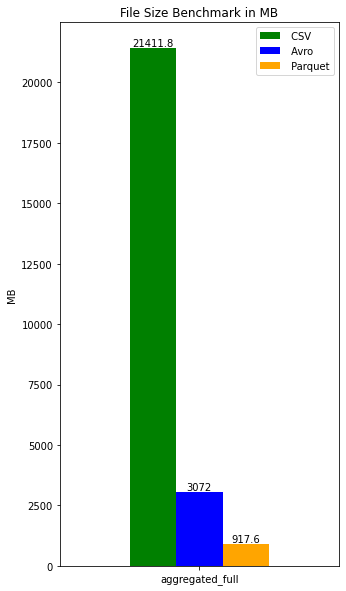
\includegraphics[width=4cm]{img/size_full.png} }}%
    \caption{File size benchmark summary of the 4 file formats in different sizes listed on the X-axis. The file size is measured in MB and shown on the Y-axis)}%
    \label{fig:size_summary}%
\end{figure}

\clearpage
\section{Discussion}
\label{sec:discussion}
This section consists of two major sections that provide an analysis of the results presented in section \ref{sec:results} and respectively, an analysis regarding the different parts of the project as well as how they may have impacted the results.

\subsection{Analysis of results}
This section presents an analysis of the results shown in Section \ref{sec:results}.
\subsubsection{Read \& Write Benchmark}
For both the read and write benchmarks with the Pandas library for textual time series data, the Parquet format has the best performance. For reading, Parquet format read time only increases by around 0.04 seconds for every 5MB increase in file size, whereas the second format in place, the csv format, has an increase of around 0.25 seconds for every 5MB increase in file size. This is most likely due to the effective columnar storage style and the compression that is done with it. Interestingly, even thus the Avro file has the same compression codec, the file size is reduced but not as much as with the Parquet file format. For a discussion on file size and compression, see \ref{sec:filestoresizesummary}. The write performance of the Parquet format is astounding since the write time does not increase with the amount of data written. Parquet also manages to give the best compression rate compared to the rest of the file formats which is shown in Figure 6 \ref{fig:size_summary}. This makes it a clear winner in this benchmark. 


\subsubsection{File stability}
The data presented in Section \ref{sect:file-stability-results} clearly shows that the csv data format experience considerably fewer reading errors and undetected effects when compared to Avro and Parquet. This is potentially due to that csv is a very redundant and uncompressed data format, which means that the randomly flipped bit is unlikely to have any meaningful impact if the flipped bit happens on the metadata or the comma used as separation. For files with compression, there is a higher probability of flipping an important bit that needs to be used to recreate and read the data correctly \cite{vohra_apache_2016_avro, shafranovich_common_2005, cao_data_2017}. The results of the file stability benchmark show that the csv data format is more resilient against file errors and undetected effects due to bit-flip when compared with Avro and Parquet. Furthermore, when comparing the number of errors and undetected effects for Avro and Parquet it can be seen that Avro experiences more errors than Parquet. Regarding the cases where there were no file reading errors, Avro resulted in more undetected effects when compared to Parquet. Since Parquet performed the best in read/write and file size performance, our research shows that there is a trade-off between file stability and read/write performance as well as file size.  

\subsubsection{File Store Size}
\label{sec:filestoresizesummary}
As shown in Figure \ref{fig:size_summary}, xlsx suffers the most in size when converted from the csv format while both Avro and Parquet show a huge file size reduction. Parquet seems to use the time series data the best since it managed to compress the 20.91 GB file into only merely 917.6MB. This is less than \(\frac{1}{20}\) when compared to the original csv file, and less than \(\frac{1}{3}\) when compared with the Avro format. This means that Parquet is once again the preferred format to its columnar storage style and the snappy compression codec.

\subsection{Discussion}
Although Parquet scored the lowest point out of the 3 file formats that were benchmarked in the file stability benchmark, the columnar-based storage format that is Parquet seems to be the best fit for textual time-series data. It has the best file size compression and read \& write performance. Therefore, one can argue that the probability that a bit flip happens in a Parquet file transfer of 917.6 MB is less likely when compared to a transfer of a csv file with a size of 20.91 GB. Not to mention the savings on hard disk space as well as network bandwidth. One may argue that when it comes to big data analysis, it is implausible that people only use Pandas for data analysis, transformation, and visualization. Tools such as Apache Spark are more likely to be used in place. Furthermore, both Avro and Parquet formats support schema in their file format as well as schema evolution. Therefore, with Spark, we can more easily and effectively check for file corruption as well as get a valid schema from the file itself. This means that for future research purposes, one should consider running the same read/write and file stability benchmarks but with Apache Spark instead of Pandas \cite{vohra_apache_2016, cao_data_2017}.

\section{Research conclusion}
\label{sec:conclusion}
Data formats are a critical component of data science pipelines to ensure high performance. Since different data formats are implemented using different technologies, they may differ in how they handle different sizes of data, which affects the performance when processing and storing the data. This means that it is of interest of understanding the potential limitations of various data formats used in data science \cite{cao_data_2017}. This research has performed a set of benchmarks to reveal potential limitations in how various data formats perform in read/write speeds, resilience against potential file errors, and file storage size. The benchmarking methodology consisted of empirically and programmatically performing benchmarks with a set of Python scripts that iteratively executes the desired operations multiple times. The results were saved for further analysis and show that Parquet is the most suitable data format when it comes to handling textual time series data. This is because Parquet achieved the lowest read/write time as well as the smallest file storage size. However, due to the compressed nature of Parquet, it performed the worst in file stability benchmarks. Therefore, there exists a trade-off between read/write performance as well as file storage size and resilience against bit-flips that cause file errors. For future research purposes, one should consider running the same read/write benchmark but with Apache Spark instead of Pandas. Additionally, other applications rather than textual time series data may be researched to better understand the differences between the data formats when used in different data science applications. 

\clearpage
\bibliography{II2202-report}
%%\bibliographystyle{IEEEtran}
\bibliographystyle{myIEEEtran}

%\clearpage
\appendix

\section{Benchmark Results}
Benchmark results are available in the results folder in the GitHub project, you can access the data via URL \href{https://github.com/emilstahl97/Research-Methodology-and-Scientific-Writing-II2202}{github.com/emilstahl97/Research-Methodology-and-Scientific-Writing-II2202}
%\subsection{Read performance benchmarks}
%\label{readappendix}
%%\begin{longtable}[h!]
  \begin{center}
    %\caption{CSV Pandas Read Benchmark}
    \label{tablecsvread}
   \pgfplotstabletypeset[
      begin table=\begin{longtable},
      end table=\end{longtable},
      %\caption{CSV Pandas Read Benchmark}
      multicolumn names, % allows to have multicolumn names
      col sep=comma, % the seperator in our .csv file
      display columns/0/.style={
        column name=$512 KB$, % name of first column
        column type={S},string type},  % use siunitx for formatting
      display columns/1/.style={
        column name=$1 MB$,
        column type={S},string type},
      display columns/2/.style={
        column name=$5 MB$,
        column type={S},string type},
      display columns/2/.style={
        column name=$5 MB$,
        column type={S},string type},
      display columns/3/.style={
        column name=$10 MB$,
        column type={S},string type},
      display columns/4/.style={
        column name=$15 MB$,
        column type={S},string type},
      display columns/5/.style={
        column name=$20 MB$,
        column type={S},string type},
      display columns/6/.style={
        column name=$Aggregated(v3-latest)$,
        column type={S},string type},
      every head row/.style={
        before row={
        \caption{CSV File Pandas Read Benchmark}%
        \endfirsthead
        \toprule
        }, % have a rule at top
        after row={%
            \si{\second} & \si{\second}& \si{\second}& \si{\second}& \si{\second}& \si{\second}& \si{\second}\\ % the units seperated by &
            \midrule} % rule under units
            },
        every last row/.style={after row=\bottomrule}, % rule at bottom
    ]{tables/csv_pandas_read_result.csv} % filename/path to file
  \end{center}
%\end{longtable}
%%\begin{longtable}[h!]
  \begin{center}
    %\caption{CSV Pandas Read Benchmark}
    \label{tablecsvread}
   \pgfplotstabletypeset[
      begin table=\begin{longtable},
      end table=\end{longtable},
      %\caption{CSV Pandas Read Benchmark}
      multicolumn names, % allows to have multicolumn names
      col sep=comma, % the seperator in our .csv file
      display columns/0/.style={
        column name=$512 KB$, % name of first column
        column type={S},string type},  % use siunitx for formatting
      display columns/1/.style={
        column name=$1 MB$,
        column type={S},string type},
      display columns/2/.style={
        column name=$5 MB$,
        column type={S},string type},
      display columns/2/.style={
        column name=$5 MB$,
        column type={S},string type},
      display columns/3/.style={
        column name=$10 MB$,
        column type={S},string type},
      display columns/4/.style={
        column name=$15 MB$,
        column type={S},string type},
      display columns/5/.style={
        column name=$20 MB$,
        column type={S},string type},
      display columns/6/.style={
        column name=$Aggregated(v3-latest)$,
        column type={S},string type},
      every head row/.style={
        before row={
        \caption{XLSX File Pandas Read Benchmark}%
        \endfirsthead
        \toprule
        }, % have a rule at top
        after row={%
            \si{\second} & \si{\second}& \si{\second}& \si{\second}& \si{\second}& \si{\second}& \si{\second}\\ % the units seperated by &
            \midrule} % rule under units
            },
        every last row/.style={after row=\bottomrule}, % rule at bottom
    ]{tables/xlsx_pandas_read_result.csv} % filename/path to file
  \end{center}
%\end{longtable}
%%\begin{longtable}[h!]
  \begin{center}
    %\caption{CSV Pandas Read Benchmark}
    \label{tablecsvread}
   \pgfplotstabletypeset[
      begin table=\begin{longtable},
      end table=\end{longtable},
      %\caption{CSV Pandas Read Benchmark}
      multicolumn names, % allows to have multicolumn names
      col sep=comma, % the seperator in our .csv file
      display columns/0/.style={
        column name=$512 KB$, % name of first column
        column type={S},string type},  % use siunitx for formatting
      display columns/1/.style={
        column name=$1 MB$,
        column type={S},string type},
      display columns/2/.style={
        column name=$5 MB$,
        column type={S},string type},
      display columns/2/.style={
        column name=$5 MB$,
        column type={S},string type},
      display columns/3/.style={
        column name=$10 MB$,
        column type={S},string type},
      display columns/4/.style={
        column name=$15 MB$,
        column type={S},string type},
      display columns/5/.style={
        column name=$20 MB$,
        column type={S},string type},
      display columns/6/.style={
        column name=$Aggregated(v3-latest)$,
        column type={S},string type},
      every head row/.style={
        before row={
        \caption{Avro File Pandas Read Benchmark}%
        \endfirsthead
        \toprule
        }, % have a rule at top
        after row={%
            \si{\second} & \si{\second}& \si{\second}& \si{\second}& \si{\second}& \si{\second}& \si{\second}\\ % the units seperated by &
            \midrule} % rule under units
            },
        every last row/.style={after row=\bottomrule}, % rule at bottom
    ]{tables/avro_pandas_read_result.csv} % filename/path to file
  \end{center}
%\end{longtable}
%%\begin{longtable}[h!]
  \begin{center}
    %\caption{CSV Pandas Read Benchmark}
    \label{tablecsvread}
   \pgfplotstabletypeset[
      begin table=\begin{longtable},
      end table=\end{longtable},
      %\caption{CSV Pandas Read Benchmark}
      multicolumn names, % allows to have multicolumn names
      col sep=comma, % the seperator in our .csv file
      display columns/0/.style={
        column name=$512 KB$, % name of first column
        column type={S},string type},  % use siunitx for formatting
      display columns/1/.style={
        column name=$1 MB$,
        column type={S},string type},
      display columns/2/.style={
        column name=$5 MB$,
        column type={S},string type},
      display columns/2/.style={
        column name=$5 MB$,
        column type={S},string type},
      display columns/3/.style={
        column name=$10 MB$,
        column type={S},string type},
      display columns/4/.style={
        column name=$15 MB$,
        column type={S},string type},
      display columns/5/.style={
        column name=$20 MB$,
        column type={S},string type},
      display columns/6/.style={
        column name=$Aggregated(v3-latest)$,
        column type={S},string type},
      every head row/.style={
        before row={
        \caption{Parquet File Pandas Read Benchmark}%
        \endfirsthead
        \toprule
        }, % have a rule at top
        after row={%
            \si{\second} & \si{\second}& \si{\second}& \si{\second}& \si{\second}& \si{\second}& \si{\second}\\ % the units seperated by &
            \midrule} % rule under units
            },
        every last row/.style={after row=\bottomrule}, % rule at bottom
    ]{tables/parquet_pandas_read_result.csv} % filename/path to file
  \end{center}
%\end{longtable}

%\clearpage
%\subsection{Write performance benchmarks}
%\label{writeappendix}


%%\begin{longtable}[h!]
  \begin{center}
    %\caption{CSV Pandas Read Benchmark}
    \label{tablecsvread}
   \pgfplotstabletypeset[
      begin table=\begin{longtable},
      end table=\end{longtable},
      %\caption{CSV Pandas Read Benchmark}
      multicolumn names, % allows to have multicolumn names
      col sep=comma, % the seperator in our .csv file
      display columns/0/.style={
        column name=$512 KB$, % name of first column
        column type={S},string type},  % use siunitx for formatting
      display columns/1/.style={
        column name=$1 MB$,
        column type={S},string type},
      display columns/2/.style={
        column name=$5 MB$,
        column type={S},string type},
      display columns/2/.style={
        column name=$5 MB$,
        column type={S},string type},
      display columns/3/.style={
        column name=$10 MB$,
        column type={S},string type},
      display columns/4/.style={
        column name=$15 MB$,
        column type={S},string type},
      display columns/5/.style={
        column name=$20 MB$,
        column type={S},string type},
      display columns/6/.style={
        column name=$Aggregated(v3-latest)$,
        column type={S},string type},
      every head row/.style={
        before row={
        \caption{CSV File Pandas Write Benchmark}%
        \endfirsthead
        \toprule
        }, % have a rule at top
        after row={%
            \si{\second} & \si{\second}& \si{\second}& \si{\second}& \si{\second}& \si{\second}& \si{\second}\\ % the units seperated by &
            \midrule} % rule under units
            },
        every last row/.style={after row=\bottomrule}, % rule at bottom
    ]{tables/csv_pandas_write_result.csv} % filename/path to file
  \end{center}
%\end{longtable}
%%\begin{longtable}[h!]
  \begin{center}
    %\caption{CSV Pandas Read Benchmark}
    \label{tablecsvread}
   \pgfplotstabletypeset[
      begin table=\begin{longtable},
      end table=\end{longtable},
      %\caption{CSV Pandas Read Benchmark}
      multicolumn names, % allows to have multicolumn names
      col sep=comma, % the seperator in our .csv file
      display columns/0/.style={
        column name=$512 KB$, % name of first column
        column type={S},string type},  % use siunitx for formatting
      display columns/1/.style={
        column name=$1 MB$,
        column type={S},string type},
      display columns/2/.style={
        column name=$5 MB$,
        column type={S},string type},
      display columns/2/.style={
        column name=$5 MB$,
        column type={S},string type},
      display columns/3/.style={
        column name=$10 MB$,
        column type={S},string type},
      display columns/4/.style={
        column name=$15 MB$,
        column type={S},string type},
      display columns/5/.style={
        column name=$20 MB$,
        column type={S},string type},
      display columns/6/.style={
        column name=$Aggregated(v3-latest)$,
        column type={S},string type},
      every head row/.style={
        before row={
        \caption{XLSX File Pandas Read Benchmark}%
        \endfirsthead
        \toprule
        }, % have a rule at top
        after row={%
            \si{\second} & \si{\second}& \si{\second}& \si{\second}& \si{\second}& \si{\second}& \si{\second}\\ % the units seperated by &
            \midrule} % rule under units
            },
        every last row/.style={after row=\bottomrule}, % rule at bottom
    ]{tables/xlsx_pandas_write_result.csv} % filename/path to file
  \end{center}
%\end{longtable}
%%\begin{longtable}[h!]
  \begin{center}
    %\caption{CSV Pandas Read Benchmark}
    \label{tablecsvread}
   \pgfplotstabletypeset[
      begin table=\begin{longtable},
      end table=\end{longtable},
      %\caption{CSV Pandas Read Benchmark}
      multicolumn names, % allows to have multicolumn names
      col sep=comma, % the seperator in our .csv file
      display columns/0/.style={
        column name=$512 KB$, % name of first column
        column type={S},string type},  % use siunitx for formatting
      display columns/1/.style={
        column name=$1 MB$,
        column type={S},string type},
      display columns/2/.style={
        column name=$5 MB$,
        column type={S},string type},
      display columns/2/.style={
        column name=$5 MB$,
        column type={S},string type},
      display columns/3/.style={
        column name=$10 MB$,
        column type={S},string type},
      display columns/4/.style={
        column name=$15 MB$,
        column type={S},string type},
      display columns/5/.style={
        column name=$20 MB$,
        column type={S},string type},
      display columns/6/.style={
        column name=$Aggregated(v3-latest)$,
        column type={S},string type},
      every head row/.style={
        before row={
        \caption{Avro File Pandas Read Benchmark}%
        \endfirsthead
        \toprule
        }, % have a rule at top
        after row={%
            \si{\second} & \si{\second}& \si{\second}& \si{\second}& \si{\second}& \si{\second}& \si{\second}\\ % the units seperated by &
            \midrule} % rule under units
            },
        every last row/.style={after row=\bottomrule}, % rule at bottom
    ]{tables/avro_pandas_write_result.csv} % filename/path to file
  \end{center}
%\end{longtable}
%%\begin{longtable}[h!]
  \begin{center}
    %\caption{CSV Pandas Read Benchmark}
    \label{tablecsvread}
   \pgfplotstabletypeset[
      begin table=\begin{longtable},
      end table=\end{longtable},
      %\caption{CSV Pandas Read Benchmark}
      multicolumn names, % allows to have multicolumn names
      col sep=comma, % the seperator in our .csv file
      display columns/0/.style={
        column name=$512 KB$, % name of first column
        column type={S},string type},  % use siunitx for formatting
      display columns/1/.style={
        column name=$1 MB$,
        column type={S},string type},
      display columns/2/.style={
        column name=$5 MB$,
        column type={S},string type},
      display columns/2/.style={
        column name=$5 MB$,
        column type={S},string type},
      display columns/3/.style={
        column name=$10 MB$,
        column type={S},string type},
      display columns/4/.style={
        column name=$15 MB$,
        column type={S},string type},
      display columns/5/.style={
        column name=$20 MB$,
        column type={S},string type},
      display columns/6/.style={
        column name=$Aggregated(v3-latest)$,
        column type={S},string type},
      every head row/.style={
        before row={
        \caption{Parquet File Pandas Read Benchmark}%
        \endfirsthead
        \toprule
        }, % have a rule at top
        after row={%
            \si{\second} & \si{\second}& \si{\second}& \si{\second}& \si{\second}& \si{\second}& \si{\second}\\ % the units seperated by &
            \midrule} % rule under units
            },
        every last row/.style={after row=\bottomrule}, % rule at bottom
    ]{tables/parquet_pandas_write_result.csv} % filename/path to file
  \end{center}
%\end{longtable}


\end{document}
